% vim:need-image-precompilation



\part{光学仪器中的衍射现象}

\section{光学仪器的分辨本领（光学衍射极限）}

\begin{slide}
  \begin{itemlist}
    \item{定义（理想分辨本领，光学衍射极限）}
      两个亮度相同、波长相等的独立光源经过理想光学系统所能达到的最佳分辨本领，也称为光学仪器分辨本领的\textbf{衍射极限}
    \item{物理图像（不确定性原理）}
      物（物点集合）$\Longrightarrow$像（像斑集合）
    \item{瑞利（Rayleigh）判据}
      设两个物点成像得到的两个艾里斑角距为$\delta\theta$，每个艾里斑的半角宽度为$\Delta\theta$；当$\delta\theta > \Delta\theta$时，可以分辨；当$\delta\theta < \Delta\theta$时，不可分辨；$\delta\theta_{\mathrm m} = \Delta\theta$称为\textbf{可分辨角极限}
  \end{itemlist}
\end{slide}

\begin{slide}
  利用圆孔夫琅禾费衍射公式估计$\Delta\theta$
  \begin{itemlist}
    \item{圆孔夫琅禾费衍射光强计算公式}
      $$
        I(\theta) = I_0\(\frac{2J_1(x)}{x}\)^2,\
        x(\theta) = \frac{\pi D\sin\theta}{\lambda}
      $$
    \item{零级斑（艾里斑）边界}
      $$
        x(\delta\theta_{\mathrm m}) = 1.22\pi\
        \Rightarrow\ \sin\delta\theta_{\mathrm m} = \frac{1.22\lambda}{D}
      $$
    \item{小角近似得到光学衍射极限}
      $$
        \delta\theta_{\mathrm m} \ll 1\
        \Rightarrow\ \boxed{\delta\theta_{\mathrm m} \approx \frac{1.22\lambda}{D}}
      $$
  \end{itemlist}
\end{slide}

\section{光学仪器的有效放大率}

\begin{slide}
  \begin{itemlist}
    \item{人眼的最小分辨角}
      白昼时瞳孔直径：$D_{\mathrm e} \sim 2\unit{mm}$ \\
      白昼时敏感波长：$\lambda \sim 550\unit{nm}$（折射率的增加使得艾里斑直径和间距等比缩小了，故没有贡献） \\
      白昼时最小分辨角：$$\boxed{\delta\theta_{\mathrm e} \approx 1.22\lambda / D_{\mathrm e} \sim 3.3 \times 10^{-4} \unit{rad} \sim 1\minute}$$
    \item{仪器的有效放大率}
      定义：$$\boxed{M_{\mathrm{eff}} = \delta\theta_{\mathrm e} / \delta\theta_{\mathrm m}}$$
      物理意义：仪器的角分辨率相比人眼提高（即可分辨角极限$\delta\theta_{\mathrm m}$降低）的倍数；仪器的最小分辨角$\delta\theta_{\mathrm m}$经仪器放大$M_{\mathrm{eff}}$倍后人眼恰好可以分辨
  \end{itemlist}
\end{slide}

\section{天文望远镜的分辨本领}

\begin{slide}
  \begin{itemlist}
    \item{目视望远镜的最小分辨角}
      目视望远镜相当于将瞳孔直径$D_{\mathrm e}$提高到望远镜物镜的大小$D_{\mathrm o}$，其最小分辨角为$\delta\theta_{\mathrm e} \approx 1.22\lambda / D_{\mathrm o}$，同时其角放大率（即物镜与目镜焦距之比）也受到仪器有效放大率$M_{\mathrm{eff}}$的限制
      \item{大型望远镜的分辨本领}
      大型望远镜的分辨本领理论上取决于其观测的波段$\lambda$和主镜的口径$D$。实际上更多取决于大气视宁度（seeing）。对于光学波段，一个口径为$10\unit{m}$的望远镜，其理论分辨角为$0.014\second$，远小于最理想的大气视宁度$\theta_s \sim 1\minute$，此时就需要使用自适应光学等技术抵消大气扰动。对于波长更长的无线电波段，即使是FAST这样的超大型望远镜最多也只有$1\minute$（在$3\unit{GHz}$下），于是人们建造望远镜阵列，通过单个望远镜之间的干涉可以将有效孔径（基线）延伸至地球大小
  \end{itemlist}
\end{slide}

\begin{slide}
    \begin{figure}[b]
        \centering
        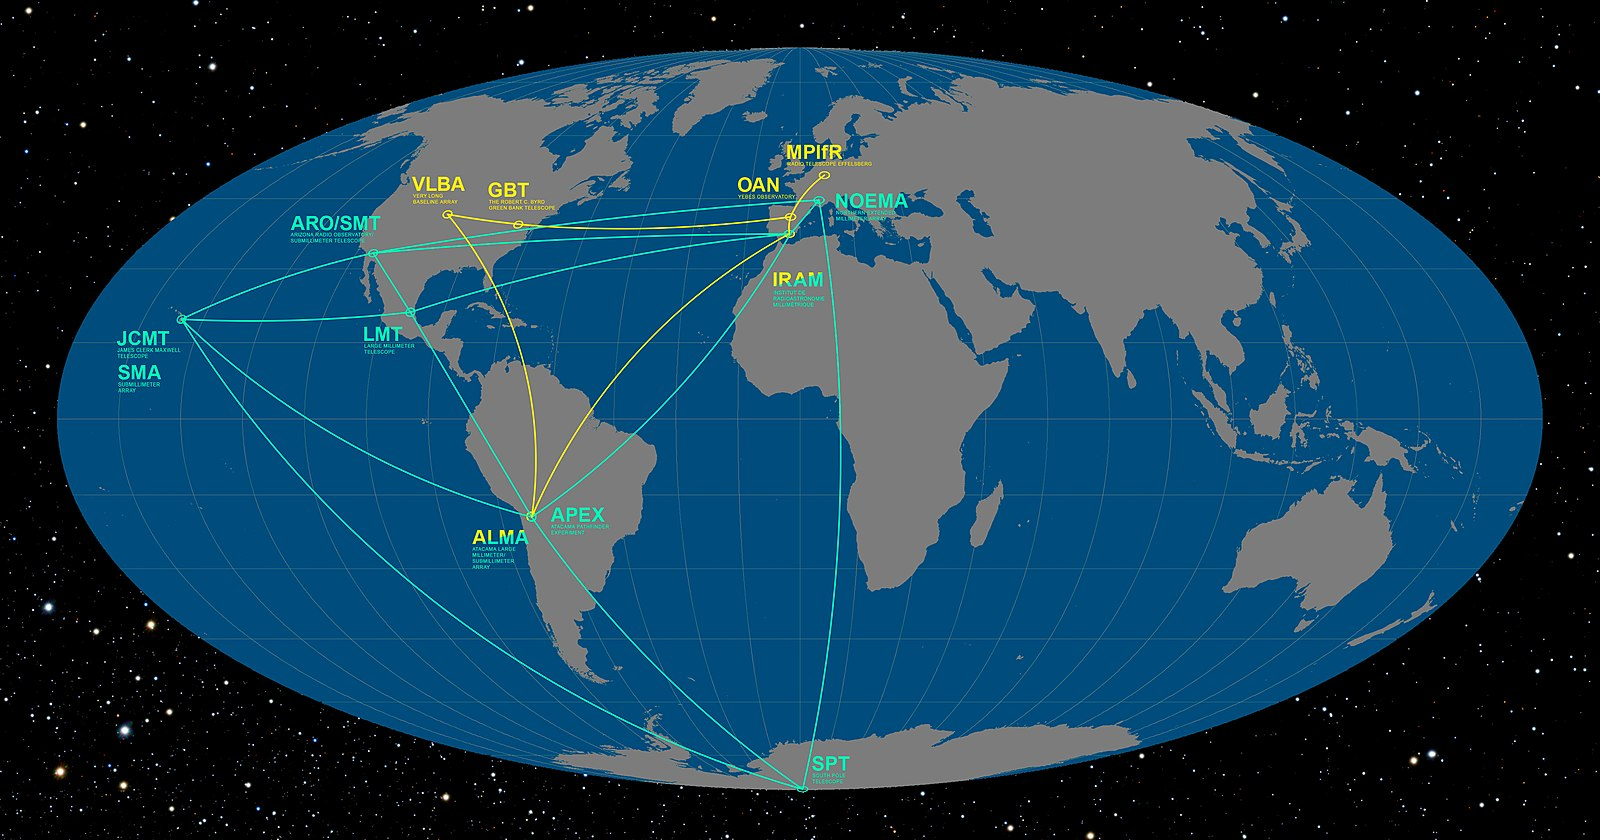
\includegraphics[height=4.5cm, width=8cm]{pictures/EHT.jpg}
        \caption{事件视界望远镜（EHT），运用甚长基线干涉技术（VLBI）使得基线长度等效于地球直径（$12742\unit{km}$），工作在$0.87\sim1.33\unit{mm}$，分辨率达到了$2\times10^{-5}\unit{arcsec}$}
       \end{figure}
  \end{slide}

\section{显微镜物镜的数值孔径}

\begin{slide}
  \begin{itemlist}
    \item{阿贝正弦条件}
      即无球差前提下傍轴物点以大孔径光束成像的充分必要条件
      $$
        \boxed{ny\sin u = n^\prime y^\prime \sin u^\prime}
      $$
      $n$：物方折射率\quad $y$：物方横向距离（远小于光线传播距离） \\
      $u$：物方孔径角（成像光束与光轴的夹角，可以很大）
    \item{数值孔径（$\mathrm{N.A.}$）的引入}
      考虑恰好可以分辨的情况，即$\Delta\theta = \delta\theta_{\mathrm m} \approx 1.22\lambda / D$ \\
      像方横向距离为$y^\prime = s^\prime\Delta\theta \approx 1.22\lambda / (D / s^\prime) \approx 0.61\lambda / \sin u^\prime$ \\
      注意到$\lambda = \lambda_0 / n^\prime$，
      所以$y^\prime \approx 0.61\lambda_0 / (n^\prime\sin u^\prime)$ \\
      结合阿贝正弦条件知
      $$
        \boxed{
          \delta y_{\mathrm m} = y \approx \frac{0.61\lambda_0}{\mathrm{N.A.}},\
          \mathrm{N.A.} := n\sin u
        }
      $$
  \end{itemlist}
\end{slide}

\begin{slide}
  \begin{itemlist}
    \item{显微镜的有效放大倍数}
      明视距离：$d_{\mathrm e} = 250\unit{mm}$ \\
      人眼通过显微镜在明视距离处看到物体的像 \\
      由光学仪器有效放大倍数的定义$M_{\mathrm{eff}} = \delta\theta_{\mathrm e} / \delta\theta_{\mathrm m}$推知
      $$
      \boxed{
        M_{\mathrm{eff}} = \frac{\delta y_{\mathrm e} / d_{\mathrm e}}{\delta y_{\mathrm m} / d_{\mathrm e}}
        % = \frac{\delta y_{\mathrm e}}{\delta y_{\mathrm m}}
        = \frac{\delta y_{\mathrm e}}{0.61\lambda_0 / \mathrm{N.A.}}
      }
      $$
      其中$\delta y_{\mathrm e} = \delta\theta_{\mathrm e}d_{\mathrm e} \sim 0.1\unit{mm}$表示人眼的线分辨本领 \\
      代表性地，取$\mathrm{N.A.} = 1.5,\ \lambda_0 = 550\unit{nm}$，得
      $$\boxed{M_{\mathrm{eff}} \sim 400}$$
      有效放大倍数从根本上限制了显微镜的分辨本领，增加放大倍数并不能突破有效放大倍数的局限
  \end{itemlist}
\end{slide}

\section{阿贝衍射极限}

\begin{slide}
  \begin{itemlist}
    \item{数值孔径的上限}
      由于$\delta y_{\mathrm m} = 0.61\lambda_0 / \mathrm{N.A.}$，大数值孔径显微镜分辨本领高 \\
      由于$\mathrm{N.A.} = n\sin u$，一般而言$\mathrm{N.A.} \leq 1.5$
    \item{阿贝衍射极限}
      结合$\delta y_{\mathrm m}$和$\mathrm{N.A.}$的表达式知，对于圆孔光学仪器，一般
      $$\boxed{\delta y_{\mathrm m} \lessapprox \lambda_0 / 2}$$
      现刻于 Ernst Abbe（1840 —— 1905）墓碑上的公式为（$d$为显微镜分辨极限，$n\sin\alpha$即为数值孔径）
      $$\boxed{d = \frac{\lambda}{2n\sin\alpha}}$$
  \end{itemlist}
\end{slide}

\section{电子显微镜}

\begin{slide}
  \begin{itemlist}
    \item{电子的波粒二象性}
      1924年德布罗意由光的波粒二象性类比猜想，实物粒子也有对应的物质波
      $$
      \begin{cases}
        \vec p = m\vec v = \hbar\vec k \\
        E = mc^2 = \hbar\omega \\
      \end{cases}
      $$
      1926年波恩的量子力学统计诠释统一了概率幅与物质波 \\
      1927年电子衍射实验验证了电子的波动性 \\
      1961年电子杨氏干涉实验进一步验证了电子的波动性
    \item{电子的德布罗意波波长}
      近代物理实验中使用的 KYKY-3200 型扫描电子显微镜加速电压最高为$U = 30\unit{kV}$，加速后电子动能$T \sim 30\unit{keV}$，静能$m_{\mathrm e}c^2 \approx 511\unit{keV} \gg T$，电子的运动是非相对论性的
      $$
      \boxed{
        \lambda \approx \frac{h}{\sqrt{2m_{\mathrm e}T}} \approx 7\unit{pm}
      }
      $$
  \end{itemlist}
\end{slide}

\begin{slide}
  \begin{itemlist}
    \item{电子光学折射率}
      光线传播的费马原理：给定起点和终点，光传播的路径$L$满足光程平稳值条件$$\delta\int_{L}n\d l = 0$$
      电子在电磁场中运动的最小作用量原理：给定起点和终点，电子运动的路径满足
      $$\delta\int_{L}\vec p \cdot \d\vec l = \delta\int_{L}p_l\d l = 0$$
      类比可知电子光学中具有折射率地位的物理量为$p_l = \vec p \cdot \vec{\hat e_l}$ \\
      以$\mu$记之，$\mu = \sqrt{2m_{\mathrm e}e\varphi\(\dfrac{e\varphi}{2m_{\mathrm e}c^2} - 1\)} + eA_l$，故
      $$
        \boxed{\mu \propto \varphi^{1 / 2},\ \text{if}\ v \ll c\ \text{and}\ A_l = 0}
      $$
  \end{itemlist}
\end{slide}

\begin{slide}
  \begin{itemlist}
    \item{电子光学折射率}
      由$\mu \propto \varphi^{1 / 2}$知，折射率与电势的二分之一次方成正比 \\
      $\mu$的变化范围比$n$大得多 \\
      限制条件：
      $$
        \nabla^2\varphi = -\rho / \epsilon,\
        \varphi_2\big|_S - \varphi_1\big|_S = 0,\
        \epsilon_2\parsh[\varphi_2]{n}\bigg|_S - \epsilon_1\parsh[\varphi_1]{n}\bigg|_S = 0
      $$
      问题：$\varphi$参考零点选择的不唯一性？
    \item{高斯轨迹方程}
      旋转对称和傍轴条件下，$V$和$B$为对称轴上的场分布，此时电子在电磁场中的运动轨迹可以用高斯轨迹方程描述：
      $$
        \newcommand{\p}{^\prime}
        \newcommand{\pp}{^{\prime\prime}}
        u\pp + \frac{V\p}{2V}u\p + \frac{V\pp + \eta^2B^2}{4V}u = 0,\
        u \in \{x, y\},\
        \eta = \(\frac{-e}{2m_{\mathrm e}}\)^{1/2}
      $$
  \end{itemlist}
\end{slide}

\begin{slide}
  \begin{itemlist}
    \item{扫描电子显微镜}
      热电子经万伏特高压加速和电磁聚焦后形成电子探针 \\
      电子探针的直径在纳米量级 \\
      电子探针在样品表面进行按行光栅状扫描 \\
      二次电子信号经聚焦和探测后转化为像素灰度 \\
      背散射电子信号作为补充
      \vspace{1em}\\\centering
      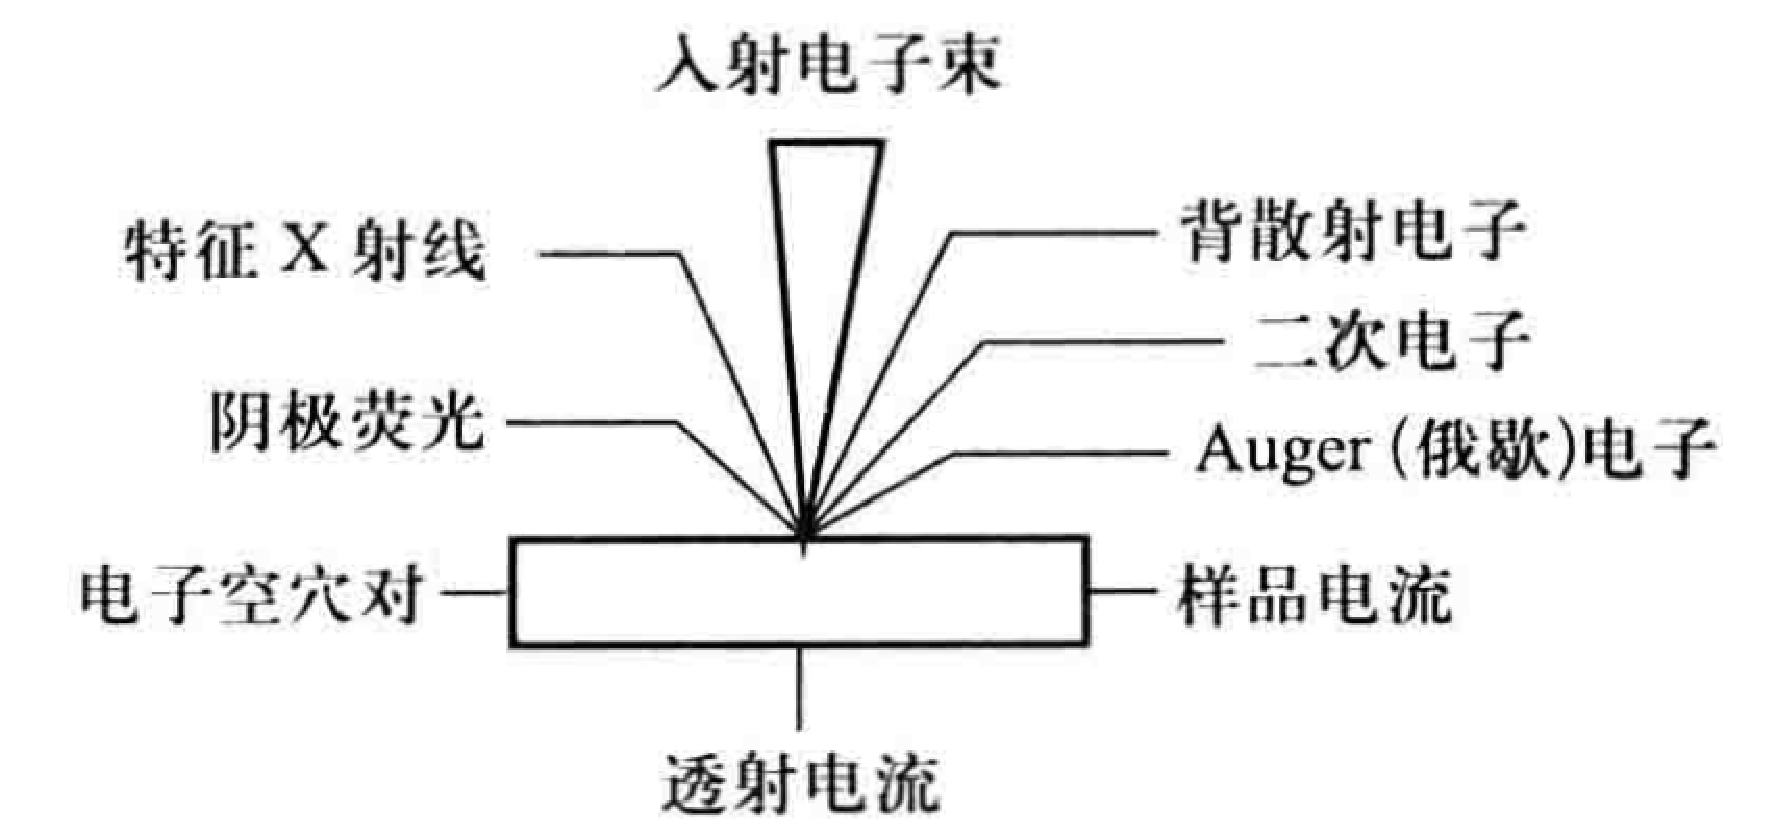
\includegraphics[width=.8\textwidth]{pictures/sem.pdf}
  \end{itemlist}
\end{slide}

\begin{slide}
  \begin{itemlist}
    \item{扫描电子显微镜下的$\chem{MgB_2}$薄膜}
      ~\\\centering
      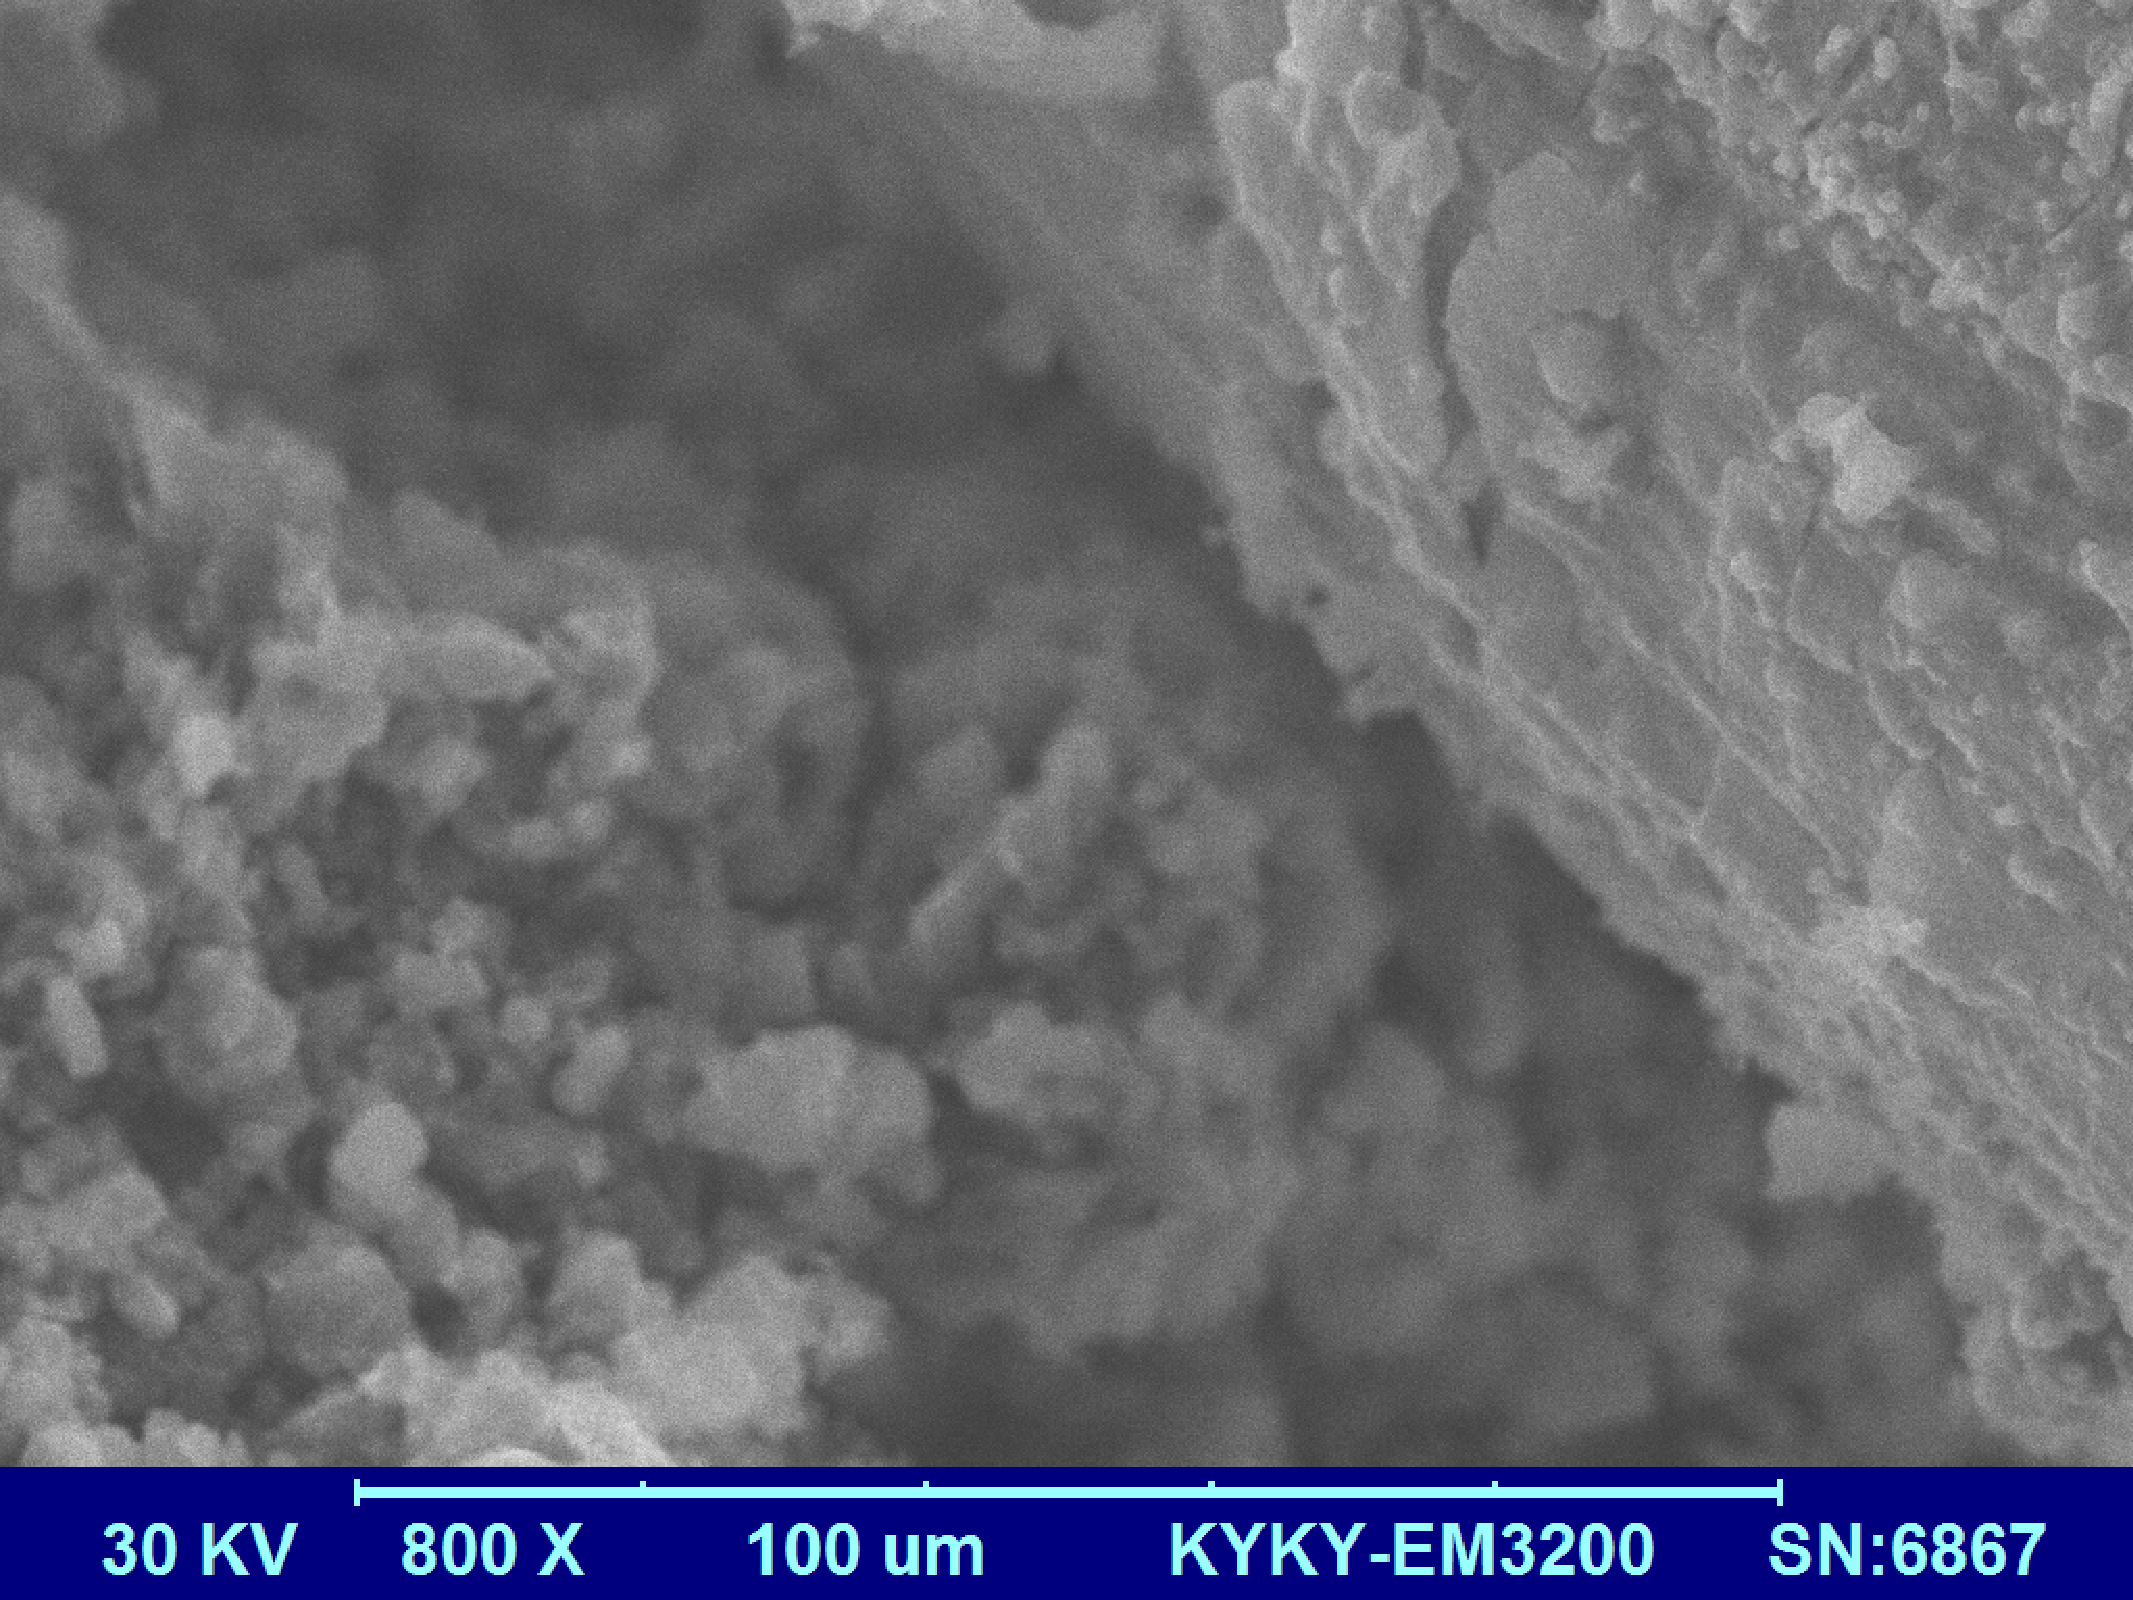
\includegraphics[width=.8\textwidth]{pictures/sem_sam.pdf}
  \end{itemlist}
\end{slide}

\begin{slide}
  \begin{itemlist}
    \item{扫描电子显微镜的分辨率}
      扫描电子显微镜的主要信号来源是\textbf{二次电子}（样品表面被入射电子照射后，逸出的价电子或弱束缚的导带电子） \\
      二次电子不可能以“大孔径”成像 \\
      其束流的发散角很小，$\sin u \approx u \sim 0.16\unit{rad}$ \\
      真空中$n = 1$，则
      $$
      \boxed{
        \delta y_{\mathrm m} \sim \frac{0.61\lambda}{0.16} \approx 4\lambda
      }
      $$
      代入$\lambda = 7\unit{pm}$有
      $$
      \boxed{
        \delta y_{\mathrm m} \sim 28\unit{pm}
      }
      $$
      实际观测发现效果不尽人意，衍射极限不是瓶颈 \\
      噪声干扰大，高放大倍数对焦困难，等等
  \end{itemlist}
\end{slide}

\section{全内反射荧光显微镜（TIRF）}

\begin{slide}
  \begin{itemlist}
    \item{TIRF (Total Internal Reflection Fluorescence)}
      隐失波穿透深度
      $$
        d_p = \frac{\lambda_0}{4\pi\sqrt{n_1^2\sin^2\theta - n_2^2}}
      $$
      典型参数$n_1 = 1.479,\ n_2 = 1.334,\ \lambda_0 = 488\unit{nm},\ \theta = 70\degree$
      $$
      \boxed{
        d_p = 100\unit{nm}
      }
      $$
      较小的“照亮”范围提供了单分子荧光蛋白成像的可能 \\
      并非突破衍射极限，而是提高了信噪比！
  \end{itemlist}
\end{slide}

\begin{slide}
  \centering
  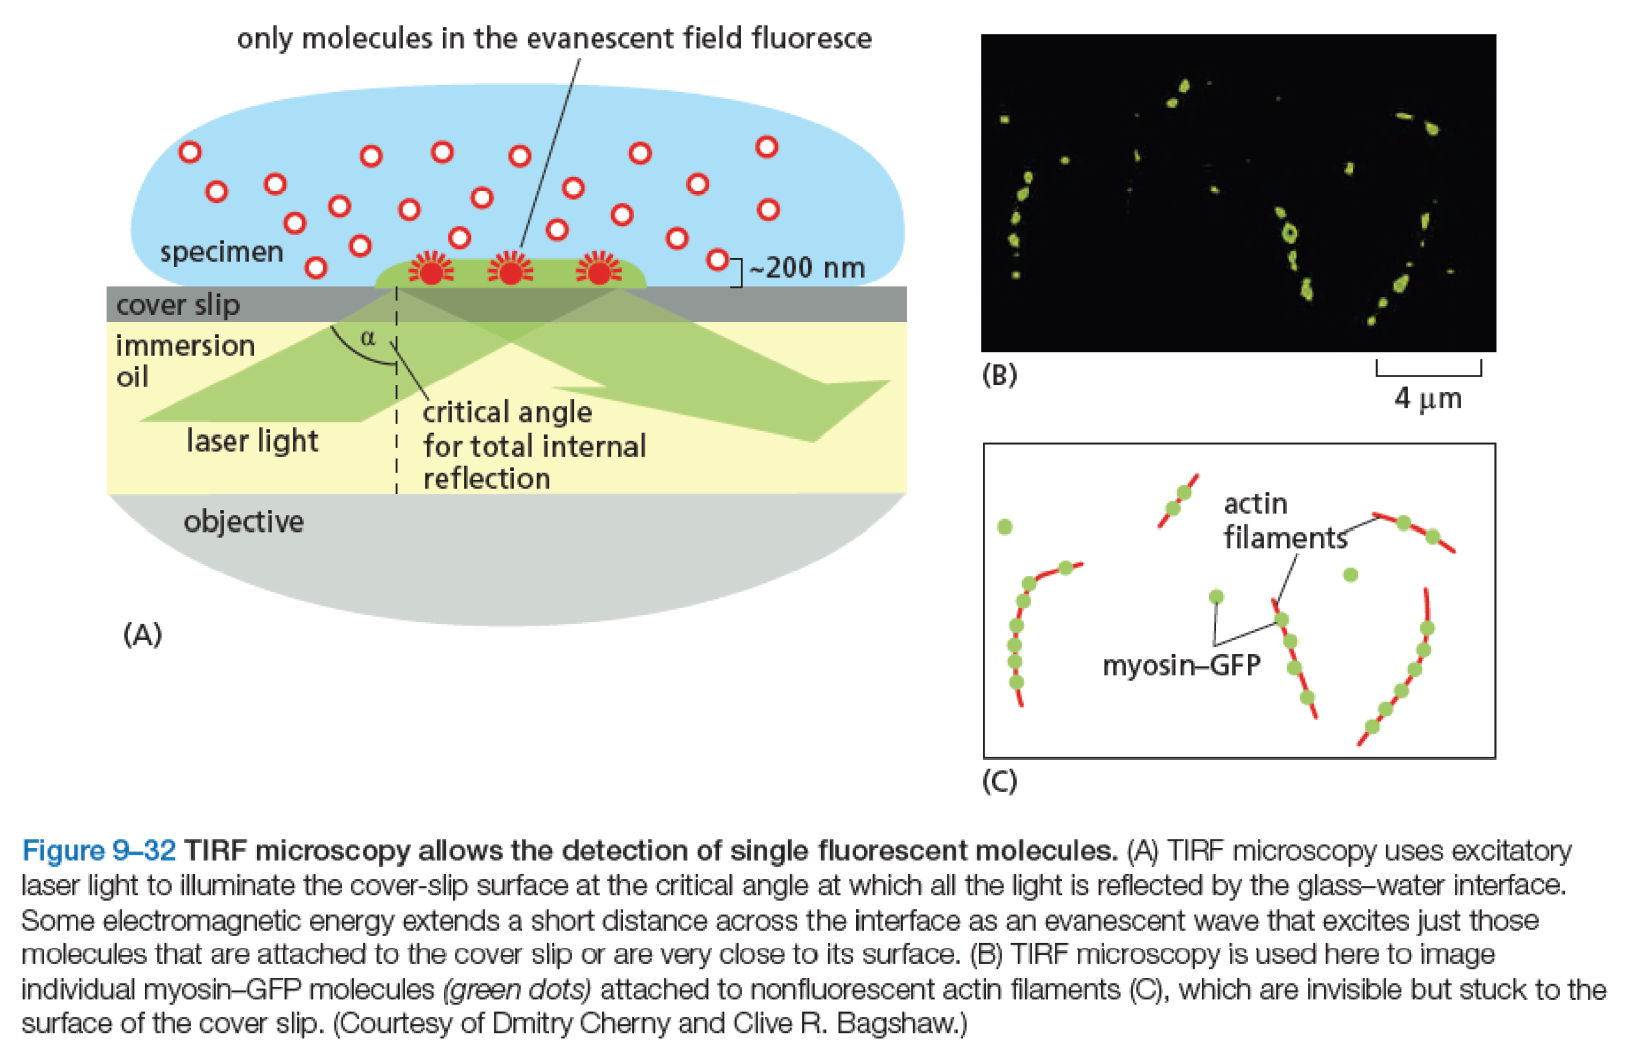
\includegraphics[width=\textwidth]{pictures/tirf.png}
\end{slide}

\section{光敏定位显微镜（PALM）和随机光学重建显微法（STORM）}
\renewcommand{\sectiontitle}{\large 光敏定位显微镜（PALM）和随机光学重建显微法（STORM）}

\begin{slide}
  \begin{itemlist}
    \item{PALM (Photoactivated Localization Microscopy)}
      分辨率：$\sim 20\unit{nm}$ \\
      使用$405\unit{nm}$ UV 调控 GFP（绿色荧光蛋白） \\
      GFP受激发后发出$488\unit{nm}$的可见光 \\
      数秒钟后即退激发 \\
      每次施加极小的激发信号 \\
      仅有少量GFP受到激发并维持数秒的暂态辐射 \\
      重复上万次（称为扫描），得到积分图像 \\
      能够尽可能地实现单分子成像，大大减少了荧光的重叠 \\
      耗时费力
    \item{\small STORM (STochastic Optical Reconstruction Microscopy)}
      类似，但扫描方式有所不同
  \end{itemlist}
\end{slide}

\begin{slide}
  \centering
  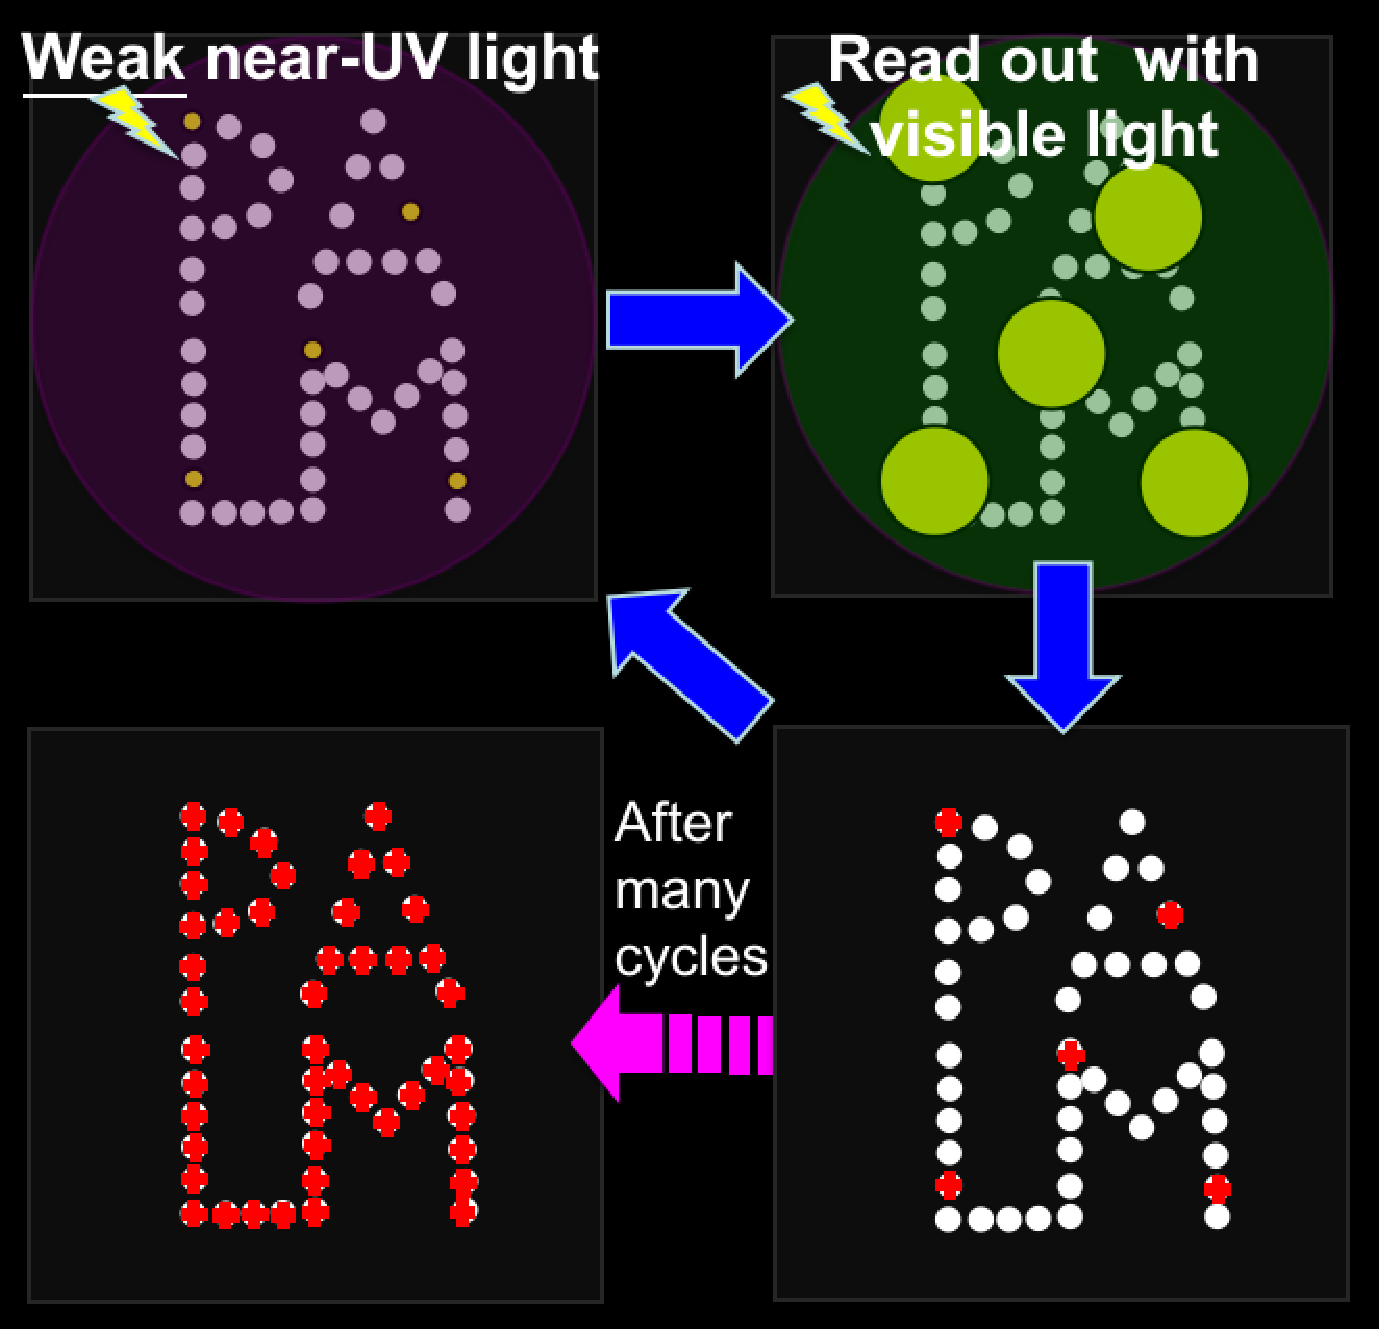
\includegraphics[width=.6\textwidth]{pictures/storm.pdf}
\end{slide}

\section{结构光照明显微镜（SIM）}

\begin{slide}
  \begin{itemlist}
    \item{SIM (Structured Illumination Microscopy)}
      分辨率：$\sim 100\unit{nm}$ \\
      相比PALM/STORM更加节能 \\
      对样品损伤小，可用于活体 \\
      高频信号混合，通过成像系统低频通带 \\
      多方向多相位成像合成重建高频信息
      \vspace{0.5em}\\\centering
      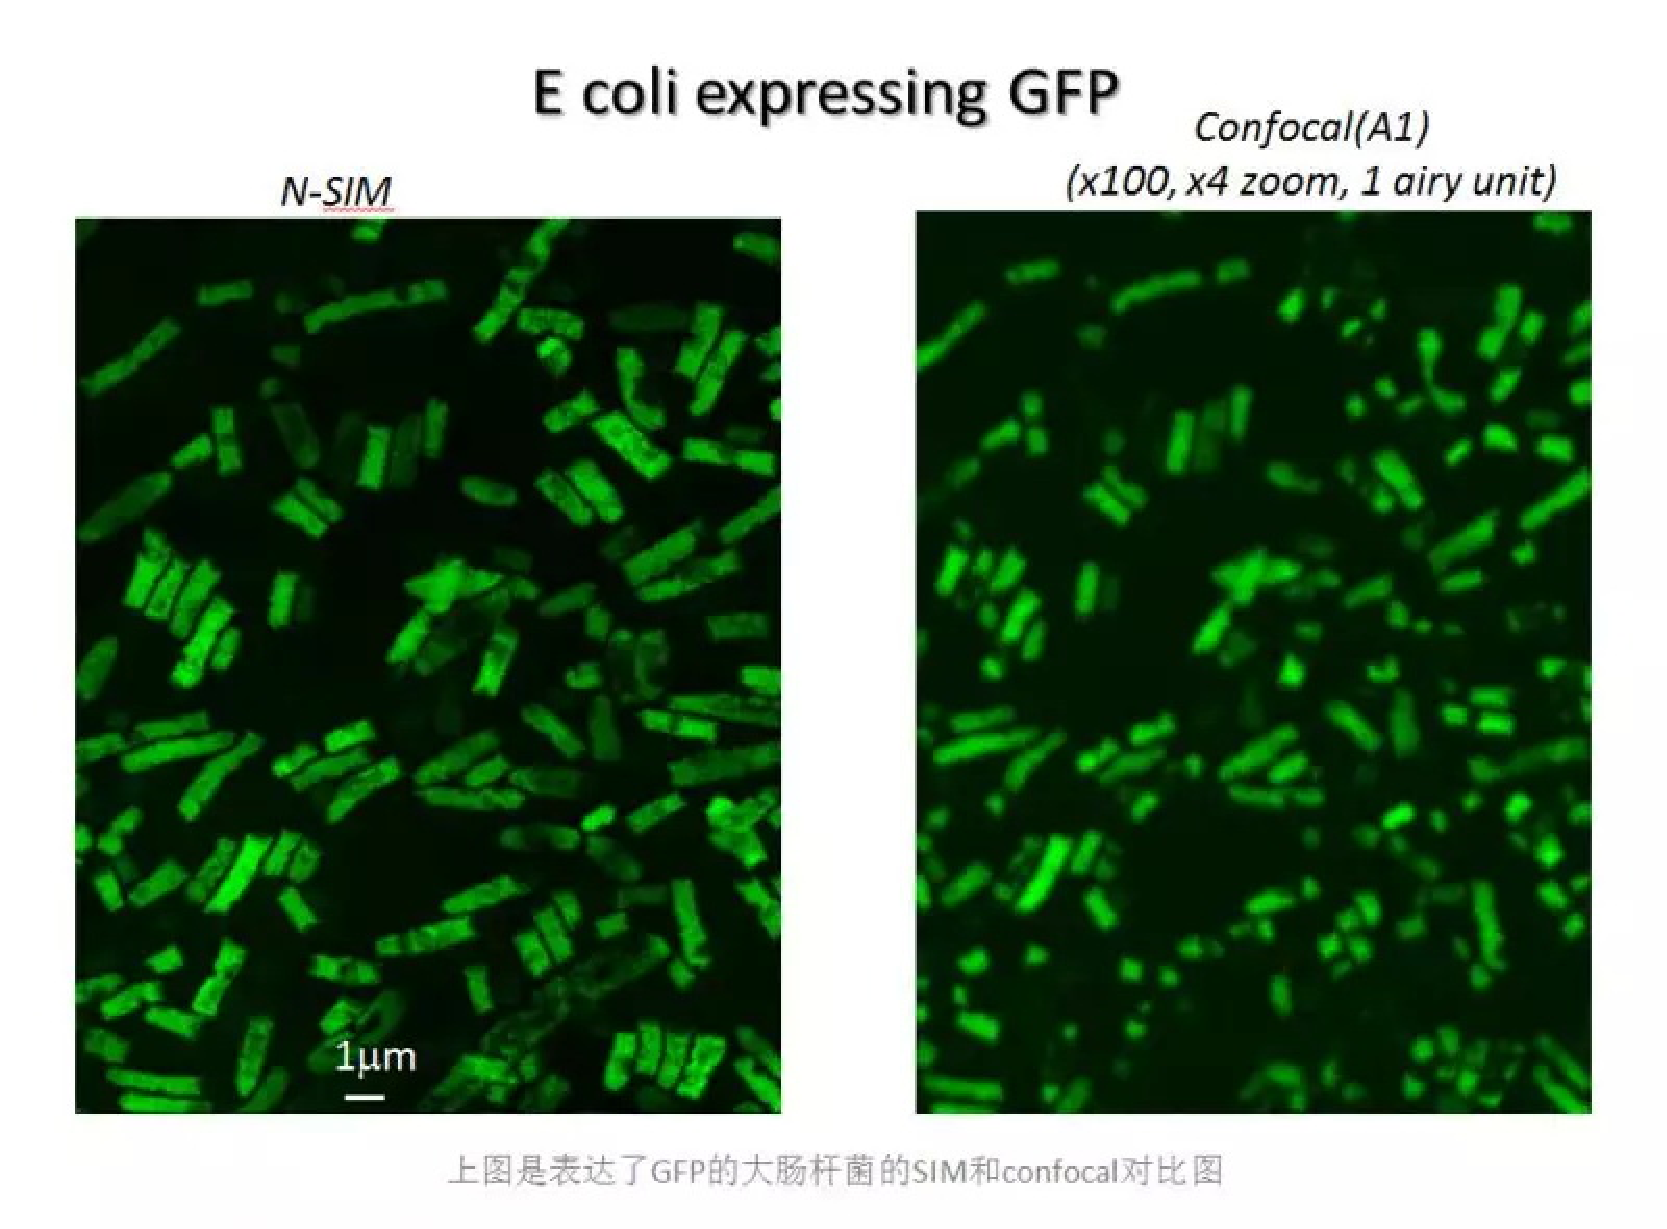
\includegraphics[width=.5\textwidth]{pictures/sim_sam.pdf}
  \end{itemlist}
\end{slide}

\begin{slide}
  \centering
  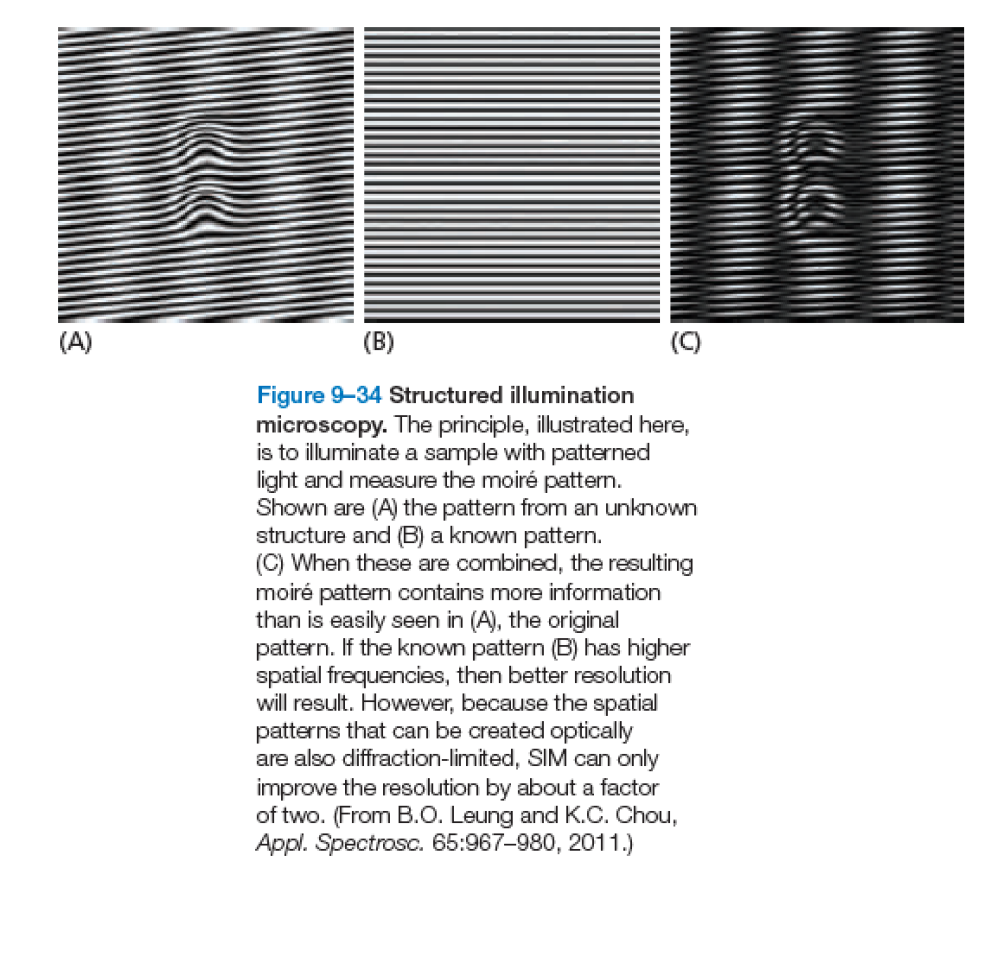
\includegraphics[width=.75\textwidth]{pictures/sim}
\end{slide}

\section{受激发射损耗荧光显微术（STED）}

\begin{slide}
  \begin{itemlist}
    \item{STED (Stimulated Emission Depletion Microscopy)}
      分辨率：$\sim 20\unit{nm}$ \\
      使用强激光使得成像荧光光斑的外围消失 \\
      高耗能
      \vspace{1em}\\\centering
      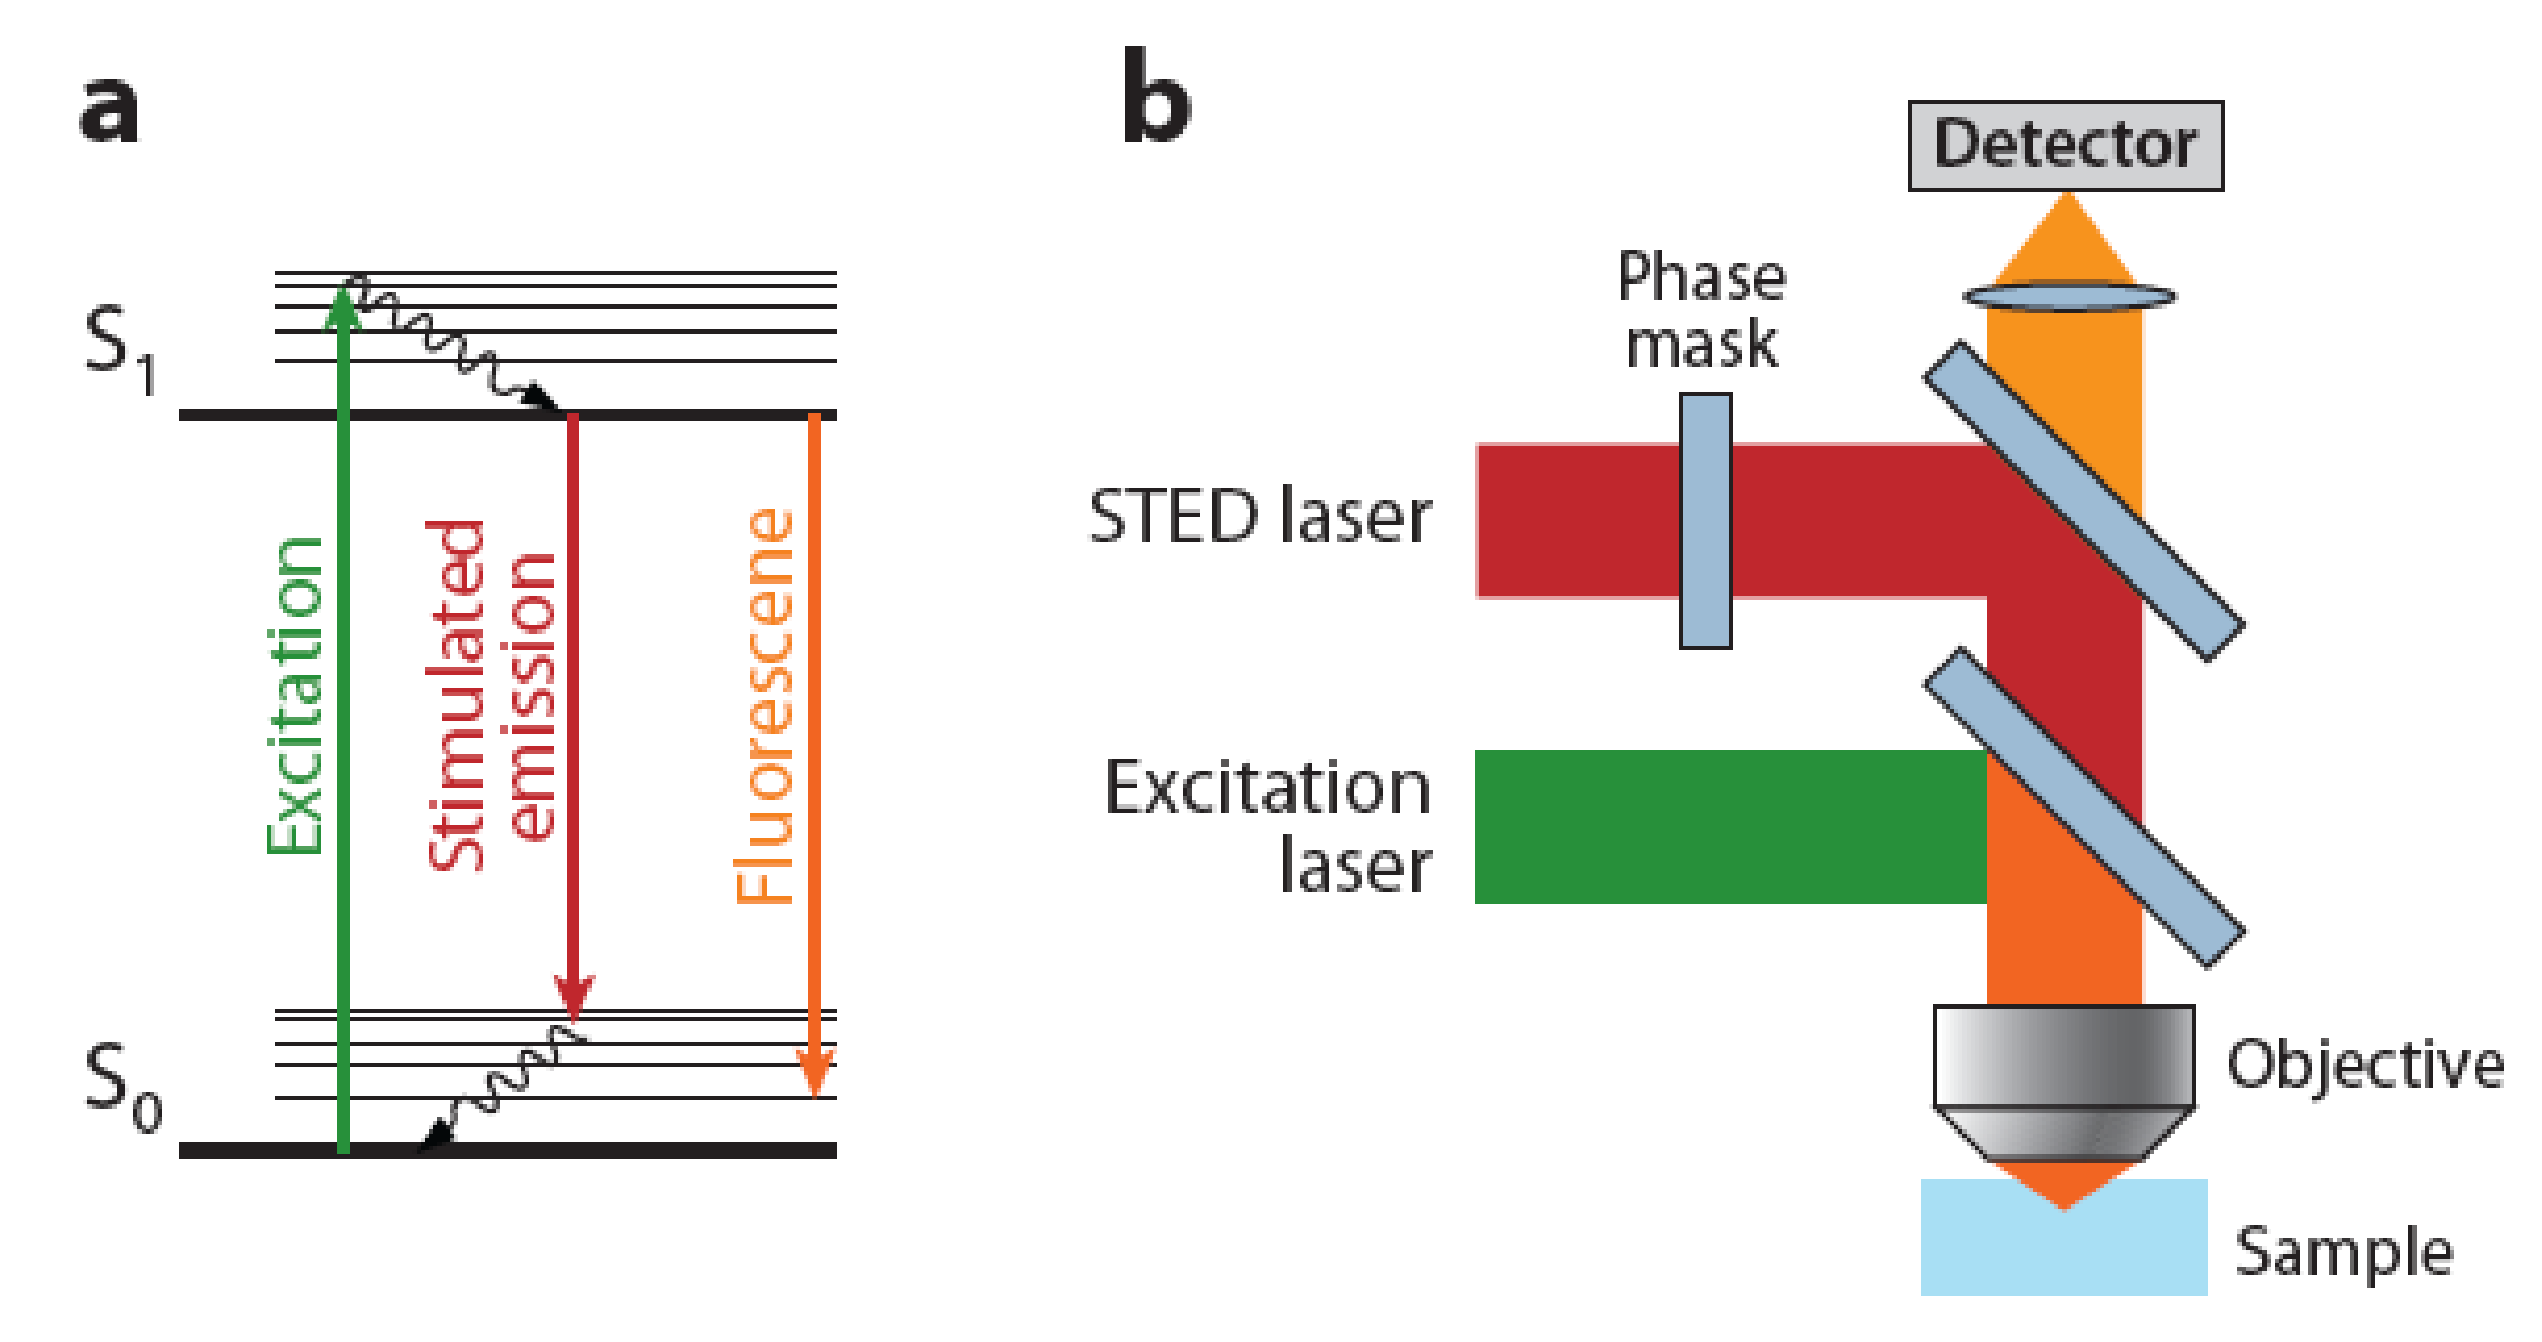
\includegraphics[width=.4\textwidth]{pictures/sted_1.pdf}
      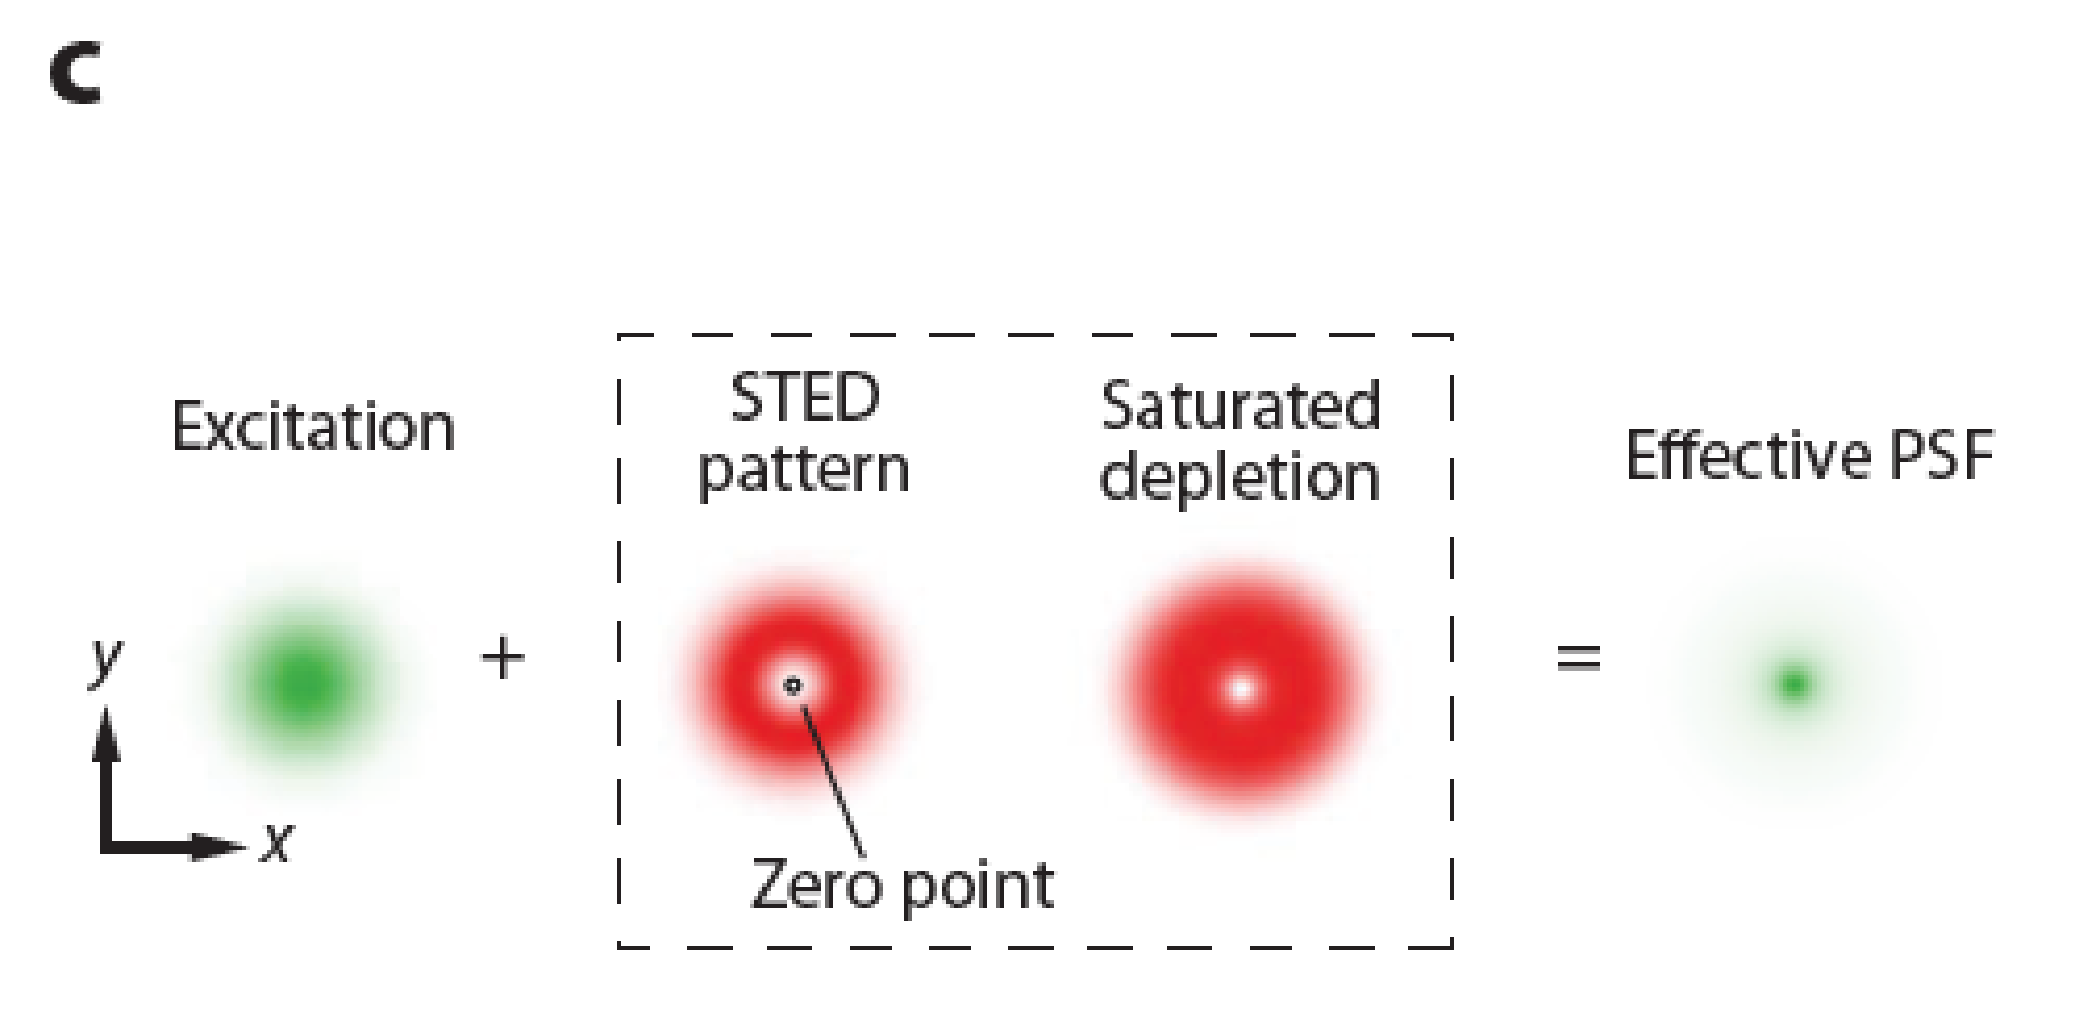
\includegraphics[width=.4\textwidth]{pictures/sted_2.pdf}
  \end{itemlist}
\end{slide}

\begin{slide}
  \centering
  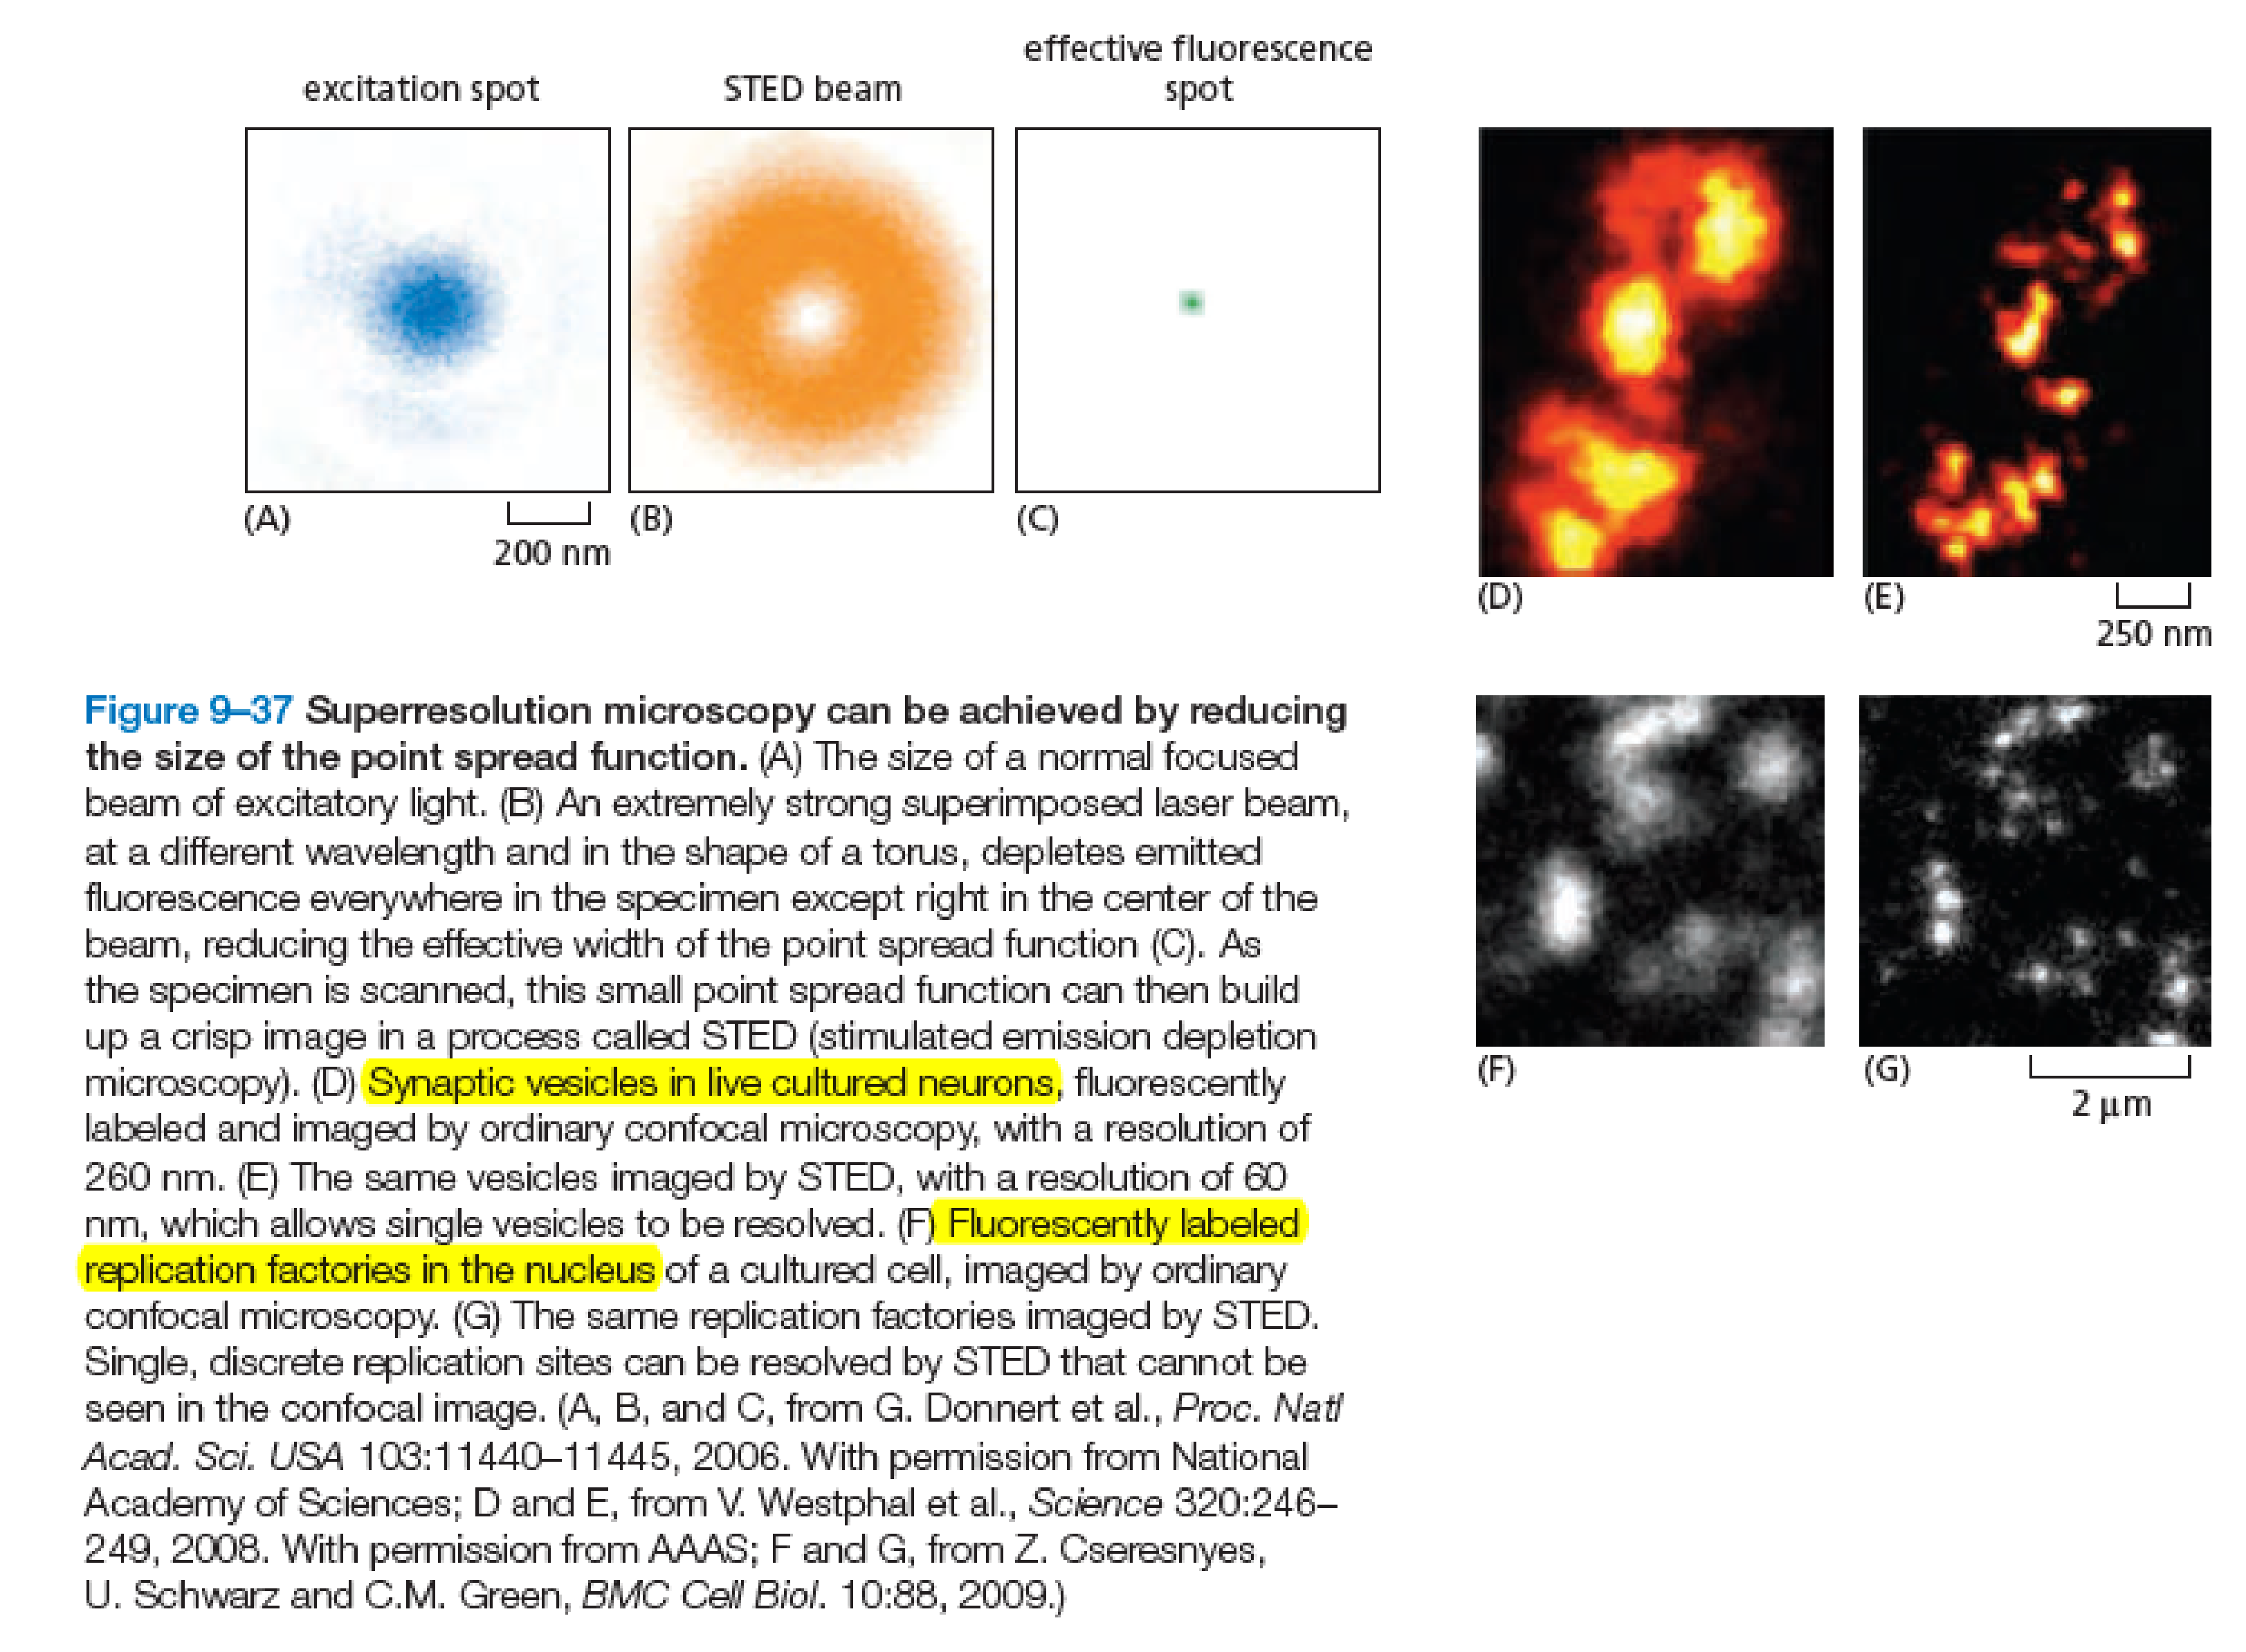
\includegraphics[width=.8\textwidth]{pictures/sted_sam.pdf}
\end{slide}
